\section{Алгоритмы обучения с подкреплением}

\subsection{Условия задачи RL}

Основной постановкой в обучении с подкреплением является задача нахождения оптимальной стратегии на основе собственного опыта взаимодействия. Это означает, что алгоритму обучения изначально доступно только:
\begin{itemize}
    \item вид пространства состояний --- количество состояний в нём в случае конечного числа, или размерность пространства $\R^d$ в случае признакового описания состояний.
    \item вид пространства действий --- непрерывное или дискретное. Некоторые алгоритмы будут принципиально способны работать только с одним из этих двух видов.
    \item взаимодействие со средой, то есть возможность для предоставленной алгоритмом стратегии $\pi$ генерировать траектории $\Traj \sim \pi$; иными словами, принципиально доступны только сэмплы из trajectory distribution \eqref{traj_expectation}.
\end{itemize}

Примерно так выглядит MDP для начинающего обучение агента:

\begin{center}
    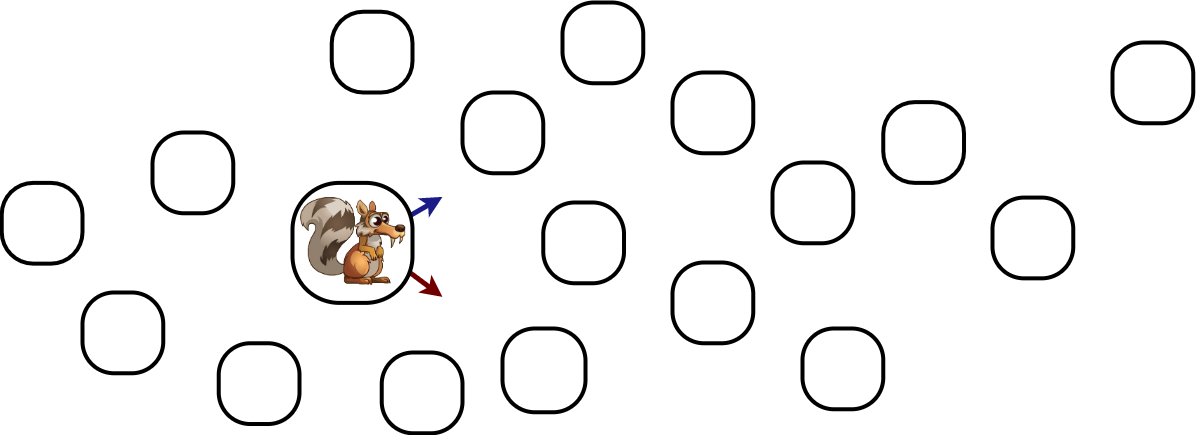
\includegraphics[width=0.9\textwidth]{Images/AgentPOV.png}
\end{center}

Итак, в отличие от обучения с учителем, где датасет <<дан алгоритму на вход>>, здесь агент должен сам собрать данные. Находясь в некотором состоянии, обучающийся агент обязан выбрать ровно одно действие, получить ровно один сэмпл $s'$ и продолжить взаимодействие (накопление опыта --- сбор сэмплов) из $s'$. Собираемые в ходе взаимодействия данные и представляют собой всю доступную агенту информацию для улучшения стратегии.

\begin{definition}
Пятёрки $\T \HM\coloneqq \left( s, a, r, s', \done \right)$, где $r \HM\coloneqq r(s, a)$, $s' \HM\sim p(s' \HM\mid s, a)$, $\done \HM\coloneqq \done(s')$, называются \emph{переходами} (transitions). 
\end{definition}

Таким образом, в RL-алгоритме должна быть прописана стратегия взаимодействия со средой во время обучения (\emph{behavior policy}), которая может отличаться от <<итоговой>> стратегии (\emph{target policy}), предназначенной для использования в среде по итогам обучения. 

% Если среда не является эпизодичной, это задача \emph{непрерывного обучения} (continual learning). Это сильно более сложная задача, хотя бы потому, что к ней можно свести ситуацию с нестационарной функцией переходов\footnote{для этого достаточно добавить в описание состояний информацию о количестве шагов всего прошедшего обучения. Понятно, что в среде с таким пространством состояний терминальных состояний быть не может.}; свойство эпизодичности позволяет RL-алгоритму пробовать разные варианты в <<одних и тех же условиях>> и обучаться за счёт их сравнения.

\subsection{On-policy vs Off-policy}

Доступной помощью для алгоритма могут быть \emph{данные от эксперта}, то есть записи взаимодействия со средой некоторой стратегии (или разных стратегий), не обязательно, вообще говоря, оптимальной. Алгоритм RL, возможно, сможет эти данные как-то использовать, или хотя бы как либо на них предобучиться. Предобучение, в простейшем случае, выглядит так: если в алгоритме присутствует параметрически заданная стратегия $\pi_\theta$, можно решать задачу \emph{имитационного обучения} (imitation learning), т.е. воспроизведения действий эксперта. Восстановление по парам $s, a$ функции $\St \HM\to \A$ --- это обычная задача обучения с учителем, однако, если эксперт не оптимален, обученная стратегия вряд ли будет действовать хоть сколько-то лучше. Понятна прямая аналогия с задачей обучения с учителем, где верхняя граница качества алгоритма определяется качеством разметки; если разметка зашумлена и содержит ошибки, обучение вряд ли удастся. В обучении с подкреплением нам не даны <<правильные действия>>, и, когда мы будем каким-либо образом сводить задачу к задачам регрессии и классификации, нам будет важно обращать внимание на то, как мы <<собираем себе разметку>> из опыта взаимодействия со средой и какое качество мы можем от этой разметки ожидать. В идеале, с каждым шагом алгоритм сможет собирать себе всё более и более <<хорошую>> разметку, за счёт неё выбирать всё более и более оптимальные действия, и так <<вытягивать сам себя из болота>>. 

\begin{definition}
Алгоритм RL называется \emph{off-policy}, если он может использовать для обучения опыт взаимодействия произвольной стратегии.
\end{definition}

\begin{definition}
Алгоритм RL называется \emph{on-policy}, если для очередной итерации алгоритма ему требуется опыт взаимодействия некоторой конкретной, предоставляемой самим алгоритмом, стратегии.
\end{definition}

Некоторое пояснение названия этих терминов: если мы обучаем некоторую стратегию $\pi$ по сэмплам любой другой произвольной стратегии $\mu$, то мы проводим <<off-policy>> обучение, обучаем политику <<не по ней же самой>>. On-policy алгоритмам будет нужно <<отправлять в среду конкретную стратегию>>, поскольку они будут способны обучать $\pi$ лишь по сэмплам из неё же самой.

Off-policy алгоритм должен уметь проводить очередной шаг обучения на произвольных траекториях, сгенерированных произвольными (возможно, разными, возможно, неоптимальными) стратегиями. Понятие принципиально важно тем, что алгоритм может потенциально переиспользовать траектории, полученные старой версией стратегии со сколь угодно давних итераций. Если алгоритм может переиспользовать опыт, но с ограничениями (например, только с недавних итераций, или только из наилучших траекторий), то мы всё равно будем относить его к on-policy. Это не означает, что для on-policy алгоритма совсем бесполезны данные от (возможно, неоптимального) эксперта; почти всегда можно придумать какую-нибудь эвристику, как воспользоваться ими для хотя бы инициализации (при помощи того же имитационного обучения). Важно, что off-policy алгоритм сможет на данных произвольного эксперта провести <<полное>> обучение, то есть условно сойтись к оптимуму при достаточном объёме и разнообразии экспертной информации, не потребовав вообще никакого дополнительного взаимодействия со средой. 

\subsection{Концепция model-free алгоритмов}

Ещё одним существенным изменением <<правил игр>> является наличие у агента прямого доступа к функции переходов $p(s' \HM\mid s, a)$ и функции награды.

\begin{definition}
Будем говорить, что у агента есть \emph{симулятор} или <<доступ к функции переходов>>, если он знает функцию награды и может в любой момент процесса обучения сэмплировать произвольное число сэмплов из $p(s' \mid s, a)$ для любого набора пар $s, a$.
\end{definition}

Симулятор --- по сути копия среды, которую агент во время обучения может откатывать к произвольному состоянию. Симулятор позволяет агенту строить свою стратегию при помощи \emph{планирования} (planning) --- рассмотрения различных вероятных версий предстоящего будущего и использования их для текущего выбора действия. При использовании планирования в идеальном симуляторе никакого процесса непосредственного обучения в алгоритме может не быть.

\begin{exampleBox}[righthand ratio=0.15, sidebyside, sidebyside align=center, lower separated=false]{}
Примером задач, в которых у алгоритма есть симулятор, являются пятнашки или кубик-рубик. То есть, пытаясь создать алгоритм, собирающий кубик-рубик, мы, естественно, можем пользоваться знаниями о том, в какую конфигурацию переводят те или иные действия текущее положение, и таким образом напрашиваются какие-то алгоритмы разумного перебора --- <<планирование>>.

\tcblower
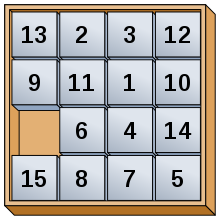
\includegraphics[width=\textwidth]{Images/puzzle.png}
\end{exampleBox}

\begin{example}
Любые задачи, в которых среда реализована виртуально, можно рассматривать как задачи, где у агента есть симулятор. Например, если мы хотим обучить бота в Марио, мы можем сказать: да у нас есть исходники кода Марио, мы можем взять любую игровую ситуацию (установить симулятор в любое состояние) и для любого действия посмотреть, что будет дальше. В RL по умолчанию считается, что в видеоиграх такого доступа нет: динамика среды изначально агенту неизвестна.
\end{example}

\begin{exampleBox}[righthand ratio=0.3, sidebyside, sidebyside align=center, lower separated=false]{}
Примером задач, в которых у алгоритма принципиально нет симулятора, являются любые задачи реальной робототехники. Важно, что даже если окружение реального робота симулируется виртуально, такая симуляция неточна --- отличается от реального мира. В таких ситуациях можно говорить, что имеется \emph{неидеальный симулятор}. Отдельно стоит уточнить, доступен ли симулятор реальному роботу в момент принятия решения (возможно, симулятор реализован на куда более вычислительно мощной отдельной системе) --- тогда он может использоваться во время обучения, но не может использоваться в итоговой стратегии.

\tcblower
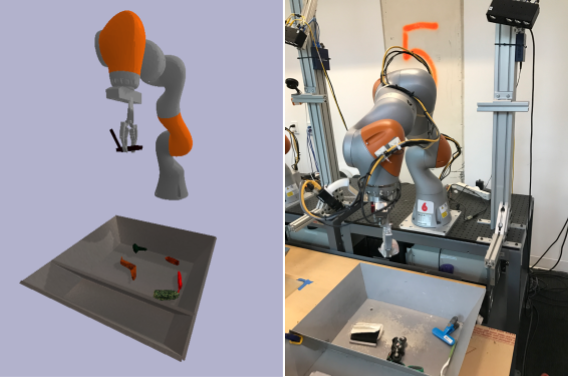
\includegraphics[width=\textwidth]{Images/realsim.png}
\end{exampleBox}

По умолчанию всегда считается, что доступа к динамике среды нет, и единственное, что предоставляется алгоритму --- среда, с которой возможно взаимодействовать. Можно ли свести такую задачу к планированию? В принципе, алгоритм может пытаться обучать себе подобный симулятор --- строить генеративную модель, по $s, a$ выдающую $s', r(s, a), \done(s')$ --- и сводить таким образом задачу к планированию. Приближение тогда, естественно, будет неидеальным.

Обучение симулятора сопряжено и с рядом других нюансов. Например, в сложных средах в описании состояний может хранится колоссальное количество информации. Построение моделей, предсказывающих будущее, может оказаться вычислительно неподъёмной и неоправданно дорогой задачей. 

Одна из фундаментальных парадигм обучения с подкреплением, вероятно, столь же важная, как парадигма end-to-end обучения для глубогоко обучения --- идея model-free обучения. Давайте не будем учить динамику среды и перебирать потенциальные варианты будущего для поиска хороших действий, а выучим напрямую связь между текущим состоянием и оптимальными действиями.

\begin{definition}
Алгоритм RL классифицируется как \emph{model-free}, если он не использует и не пытается выучить модель динамики среды $p(s' \HM\mid s, a)$. 
\end{definition}

\subsection{Классификация RL-алгоритмов}

При рассмотрении алгоритмов RL мы начнём с рассмотрения именно model-free алгоритмов и большую часть времени посвятим им. Их часто делят на следующие подходы:
\begin{itemize}
    \item \emph{мета-эвристики} (metaheuristic) никак не используют внутреннюю структуру взаимодействия среды и агента, и рассматривают задачу максимизации $J(\pi)$ как задачу <<black box оптимизации>>: можно примерно оценивать, чему равно значение функционала для разных стратегий, а структура задачи --- формализм MDP --- не используется; мы рассмотрим мета-эвристики в главе \ref{metaheuristicchapter} как не требующие построения особой теории. 
    \item \emph{value-based} алгоритмы получают оптимальную стратегию неявно через теорию оценочных функций, которую мы рассмотрим в главе \ref{classictheorychapter}. Эта теория позволит нам построить value-based алгоритмы (глава \ref{valuebasedchapter}) и будет использоваться всюду далее.
    \item \emph{policy gradient} алгоритмы максимизируют $J(\pi)$, используя оценки градиента функционала по параметрам стратегии; мы сможем помочь процессу оптимизации, правильно воспользовавшись оценочными функциями (глава \ref{policygradientchapter}).
\end{itemize}

Затем в главе \ref{continuouscontrolchapter} мы отдельно обсудим несколько алгоритмов специально для непрерывных пространств действий, находящихся на стыке value-based и policy gradient подхода, и увидим, что между ними довольно много общего. Наконец, \emph{model-based} алгоритмы, которые учат или используют предоставленную модель среды $p(s' \HM\mid s, a)$, и которые обычно выделяют в отдельную категорию, будут рассмотрены после в главе \ref{modelbasedchapter}.

\subsection{Критерии оценки RL-алгоритмов}

При оценивании алгоритмов принципиально соотношение трёх критериев:
\begin{itemize}
    \item \emph{performance}: Монте-Карло оценка значения $J(\pi)$;
    \item \emph{wall-clock time}: реальное время работы, потребовавшееся алгоритму для достижения такого результата (в полной аналогии с классическими методами оптимизации);
    \item \emph{sample efficiency}: количество сэмплов (или шагов) взаимодействия со средой, потребовавшихся алгоритму. Этот фактор может быть ключевым, если взаимодействие со средой дорого (например, обучается реальный робот); 
\end{itemize}

\begin{remark}Поскольку \href{https://openai.com/projects/five/}{победами над кожаными мешками в дотах} уже никого не удивишь, вторые два фактора начинают играть всю большую роль.
\end{remark}

В отличие от классических методов оптимизации, речи о критерии останова идти не будет, поскольку адекватно разумно проверить около-оптимальность текущей стратегии не представляется возможным в силу слишком общей постановки задачи. Считается, что оптимизация (обучение за счёт получения опыта взаимодействия) происходит, пока доступны вычислительные ресурсы; в качестве итога обучения предоставляется или получившаяся стратегия, или наилучшая встречавшаяся в ходе всего процесса.

\subsection{Сложности задачи RL}

Обсудим несколько <<именованных>> проблем задачи обучения с подкреплением, с которыми сталкивается любой алгоритм решения.

Проблема \emph{застревания в локальных оптимумах} приходит напрямую из методов оптимизации. В оптимизируемом функционале \eqref{goal} может существовать огромное количество стратегий $\pi$, для которых его значение далеко не максимально, но все в некотором смысле <<соседние>> стратегии дают в среднем ещё меньшую награду.

\begin{exampleBox}[righthand ratio=0.25, sidebyside, sidebyside align=center, lower separated=false]{}
Часто агент может выучить тривиальное <<пассивное>> поведение, которое не приносит награды, но и позволяет избегать какие-то штрафов за неудачи. Например, агент, который хочет научиться перепрыгивать через грабли, чтобы добраться до тортика (+1), может несколько раз попробовать отправиться за призом, но наступить на грабли (-1), и выучить ничего не делать (+0). Ситуация весьма типична: например, Марио может пару раз попробовать отправиться покорять первый уровень, получить по башке и решить не ходить вправо, а тупить в стену и получать <<безопасный>> +0. Для нашей задачи оптимизации это типичнейшие локальные экстремумы: <<похожие стратегии>> набирают меньше текущей, и, чтобы добраться до большей награды, нужно как-то найти совершенно новую область в пространстве стратегий.

\tcblower

\includegraphics[width=\textwidth]{Images/MarioStupid.png}
\end{exampleBox}

Другие проблемы куда более характерны именно для RL. Допустим, агент совершает какое-то действие, которое запускает в среде некоторый процесс. Процесс протекает сам по себе без какого-либо дальнейшего вмешательства агента и завершается через много шагов, приводя к награде. Это проблема \emph{отложенного сигнала} (delayed reward) --- среда даёт фидбэк агенту спустя какое-то (вообще говоря, неограниченно длительное) время.

\begin{exampleBox}[righthand ratio=0.25, sidebyside, sidebyside align=center, lower separated=false]{}
Пример из видеоигр --- в игре Atari Space Invaders очки даются в момент, когда удачный выстрел попал во вражеское НЛО, а не когда агент этот выстрел, собственно, совершает. Между принятием решения и получением сигнала проходит до нескольких секунд, и за это время агент принимает ещё несколько десятков решений.

\tcblower
\includegraphics[width=\textwidth]{Images/SpaceInvaders.png}
\end{exampleBox}

Смежная проблема --- какое именно из многих совершённых агентом действий привело к сигналу награды? \emph{Credit assignment problem} --- даже для уже собранного опыта может быть тяжело оценить, какие действия были правильными, а какие нет. 

\begin{example}
Вы поймали скунса, сварили яичницу, завезли банку горчицы в ближайший магазин штор, написали научную статью про шпроты, накормили скунса яичницей, сыграли в боулинг глобусом, вернулись домой после тяжёлого дня и получили +1. Вопрос: чему вы научились? 
\end{example}

Поскольку функция награды может быть произвольная, довольно типично, когда сигнал от среды --- неконстантная награда за шаг --- приходит очень редко. Это проблема \emph{разреженной награды} (sparse reward).

\begin{exampleBox}[righthand ratio=0.15, sidebyside, sidebyside align=center, lower separated=false]{Mountain Car}
\href{https://gym.openai.com/envs/MountainCar-v0/}{Визуализация задачи в OpenAI Gym}: тележка хочет забраться на горку, но для этого необходимо поехать в противоположном направлении, чтобы набрать разгона. Состояния описываются двумя числами (x-координата тележки и её скорость); действий три (придать ускорения вправо, влево, или ничего не делать). Функция награды равна -1 всюду: задачей агента является как можно скорее завершить эпизод. Однако, терминальное состояние --- это вершина горки, и для того, чтобы достичь его, нужно <<уже уметь>> задачу решать.  

\tcblower
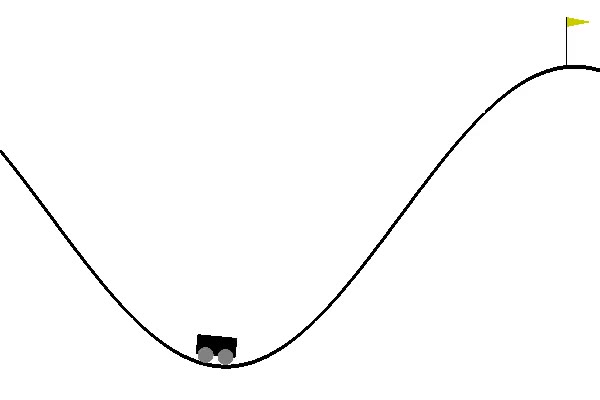
\includegraphics[width=\textwidth]{Images/MC.jpg}
\end{exampleBox}

Наконец, проблема, обсуждению которой мы посвятим довольно много времени --- \emph{дилемма исследования-использования} (exploration-exploitation trade-off). Пока ограничимся лишь примером для иллюстрации.

\begin{example}
Вы решили пойти сегодня в ресторан. Следует ли отправится в ваш любимый ресторан, или попробовать новый, в котором вы ещё ни разу не были?
\end{example}

Практическая проблема, отчасти связанная с тем, что алгоритму необходимо постоянно <<пробовать новое>> --- проблема \emph{<<безопасного обучения>>} (Safe RL). Грубо говоря, некоторые взаимодействия агента со средой крайне нежелательны даже во время обучения, в том числе когда агент ещё только учится. Эта проблема возникает в первую очередь для реальных роботов.

\begin{example}
Вы хотите научить реального робота мыть посуду. В начале обучения робот ничего не умеет и рандомно размахивает конечностями, бьёт всю посуду, переворачивает стол, сносит все лампочки и <<в исследовательских целях>> самовыкидывается из окна. В результате, начать второй обучающий эпизод становится довольно проблематично.
\end{example}

\begin{remark}
Здесь надо помнить, что безопасный RL не о том, как <<не сбивать пешеходов>> при обучении автономных автомобилей; он о том, как сбивать меньше пешеходов. RL по определению обучается на собственном опыте и в том числе собственных ошибках, и эти ошибки ему либо нужно совершить, либо получить в форме некоторой априорной информации (экспертных данных), хотя последнее всё равно не защищает от дальнейших исследований любых областей пространства состояний. Это означает, что на практике единственная полноценная защита от нежелательного поведения робота может быть проведена исключительно на этапе построения среды. То есть среда должна быть устроена так, что робот в принципе не может совершить нежелательных действий: опасные ситуации должны детектироваться средой (то есть --- внешне, внешним отдельным алгоритмом), а взаимодействие --- прерываться (с выдачей, например, отрицательной награды для агента).
\end{remark}

\begin{remark}
Одна из причин распространения видеоигр для тестирования RL --- отсутствие проблемы Safe RL: не нужно беспокоиться о том, что робот <<что-то сломает>> в процессе сбора опыта, если среда уже задана программной симуляцией.
\end{remark}

И ещё одна, вероятно, главная проблема\footnote{а точнее, в принципе главная проблема всей нашей жизни (what is your reward function?)}. \emph{Откуда берётся награда?} Алгоритмы RL предполагают, что награда, как и среда, заданы, <<поданы на вход>>, и эту проблему наши алгоритма обучения, в отличие от предыдущих, решать идеологически не должны. Но понятно, что если для практического применения обучения с учителем боттлнеком часто является необходимость размечивать данные --- <<предоставлять обучающий сигнал>> --- то в RL необходимо аккуратно описать задачу при помощи функции награды.

\begin{definition}
<<\emph{Reward hypothesis}>>: любую интеллектуальную задачу можно задать (определить) при помощи функции награды.
\end{definition}

В обучении с подкреплением принято полагать эту гипотезу истинной. Но так ли это? RL будет оптимизировать ту награду, которую ему предоставят, и дизайн функции награды в ряде практических задач оказывается проблемой.

\begin{example}[<<Взлом>> функции награды]
\href{https://www.youtube.com/watch?v=tlOIHko8ySg}{Классический пример того}, как RL оптимизирует не то, что мы ожидаем, а ту награду, которую ему подсунули. Причина зацикливания агента видна в нижнем левом углу, где отображается счёт игры.
\end{example}

\begin{example}
Попробуйте сформулировать функцию награды для следующих интеллектуальных задач:
\begin{itemize}
    \item очистка мебели от пыли;
    \item соблюдение правил дорожного движения автономным автомобилем;
    \item захват мира;
\end{itemize}
\end{example}

\subsection{Бенчмарки}

Для тестирования RL алгоритмов есть несколько распространившихся бенчмарков. Неистощаемым источником тестов для обучения с подкреплением с дискретным пространством действий являются видеоигры, где, помимо прочего, уже задана функция награды --- счёт игры.

\begin{example}[Игры Atari]
Atari --- набор из 57 игр с дискретным пространством действий. Наблюдением является экран видео-игры (изображение), у агента имеется до 18 действий (в некоторых играх действия, соответствующие бездействующим кнопкам джойстика, по умолчанию убраны). Награда --- счёт в игре. \href{https://gym.openai.com/envs/#atari}{Визуализация игр из OpenAI Gym}.

\needspace{12\baselineskip}
\begin{wrapfigure}{r}{0.4\textwidth}
\centering
\vspace{-0.3cm}
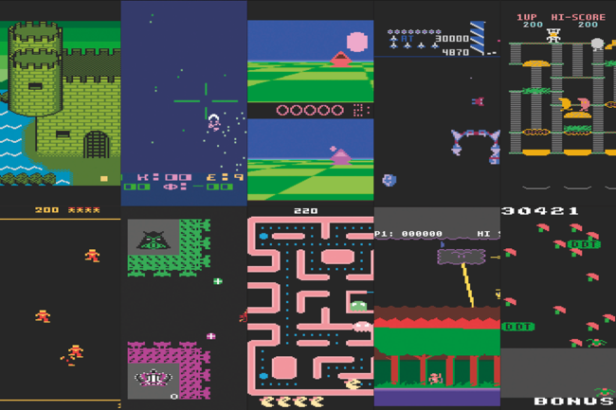
\includegraphics[width=0.4\textwidth]{Images/Atari.png}
\vspace{-0.8cm}
\end{wrapfigure}

При запуске алгоритмов на Atari обычно используется препроцессинг. В общем случае MDP, заданное исходной игрой, не является полностью наблюдаемым: например, в одной из самых простых игр Pong текущего экрана недостаточно, чтобы понять, в какую сторону летит шарик. Для борьбы с этим состоянием считают последние 4 кадра игры (\emph{frame stack}), что для большинства игр достаточно.

Чтобы агент не имел возможности менять действие сильно чаще человека, применяют \emph{frame skip} --- агент выбирает следующее действие не каждый кадр, а, скажем, раз в 4 кадра. В течение этих 4 кадров агент нажимает одну и ту же комбинацию кнопок. Если агент <<видит>> из-за этого только кратные кадры, могут встретиться неожиданные последствия: например, в Space Invaders каждые 4 кадра <<исчезают>> все выстрелы на экране, и агент может перестать их видеть.

\begin{remark}
Обычно добавляется и препроцессинг самого входного изображения --- в оригинале оно сжимается до размера 84х84 и переводится в чёрно-белое.
\end{remark}

\begin{remark}
В играх часто встречается понятие <<жизней>>. Полезно считать, что потеря жизни означает конец эпизода и выдавать в этот момент алгоритму флаг $\done$. 
\end{remark}

Функция переходов в Atari --- детерминированная; рандомизировано только начальное состояние. Есть опасения, что это может приводить к <<запоминанию>> хороших траекторий, поэтому распространено использование \emph{sticky actions} --- текущее выбранное действие повторяется для $k$ кадров, где $k$ определяется случайно (например, действие повторяется только 2 раза, затем для очередного кадра подбрасывается монетка, и с вероятностью 0.5 агент повторяет действие снова; монетка подбрасывается снова, и так далее, пока не выпадет останов).

Для оценки алгоритмов используется \emph{Human normalized score}: пусть $\mathrm{agentScore}$ --- полученная оценка $J(\pi)$ для обучившегося агента, $\mathrm{randomScore}$ --- случайной стратегии, $\mathrm{humanScore}$ --- средний результат человека, тогда Human normalized score равен
$$\frac{\mathrm{agentScore} - \mathrm{randomScore}}{\mathrm{humanScore} - \mathrm{randomScore}}.$$
Эта величина усредняется по 57 играм для получения качества алгоритма. При этом по условию бенчмарка алгоритм должен быть запущен на всех 57 играх с одними и теми же настройками и гиперпараметрами.
\end{example}

\begin{example}[Atari RAM]
Игры Atari представлены в ещё одной версии --- <<RAM-версии>>. Состоянием считается не изображение экрана, а 128 байт памяти Atari-консоли, в которой содержится вся информация, необходимая для расчёта игры (координаты игрока и иные параметры). По определению, такое состояние <<полностью наблюдаемое>>, и также может использоваться для тестирования алгоритмов.
\end{example}

Для задач непрерывного управления за тестовыми средами обращаемся к физическим движкам и прочим симуляторам. Здесь нужно оговориться, что схожие задачи в разных физических движках могут оказаться довольно разными, в том числе по сложности для RL алгоритмов.

\begin{example}
Задача научить ходить какое-нибудь существо весьма разнообразна. Под <<существом>> понимается набор сочленений, каждое из которых оно способно <<напрягать>> или <<расслаблять>> (для каждого выдаётся вещественное число в диапазоне $[-1, 1]$). Состояние обычно описано положением и скоростью всех сочленений, то есть является небольшим компактным векторочком. 

\needspace{10\baselineskip}
\begin{wrapfigure}{r}{0.25\textwidth}
\centering
\vspace{-0.3cm}
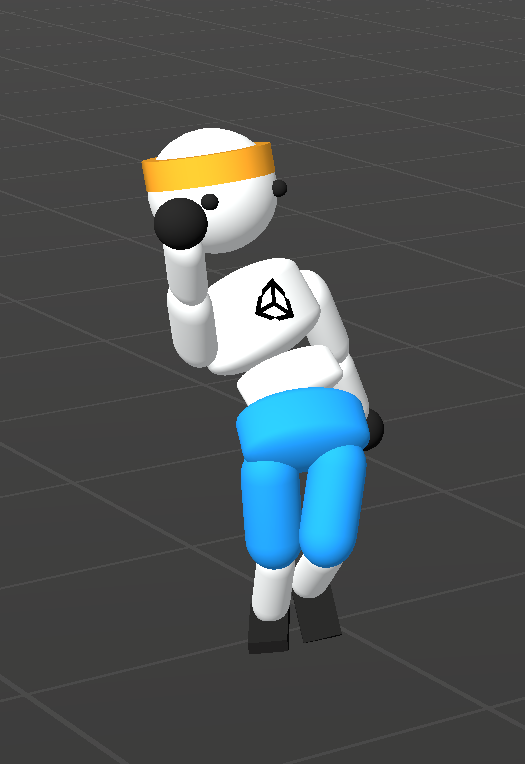
\includegraphics[width=0.25\textwidth]{Images/Dancer.png}
\vspace{-0.8cm}
\end{wrapfigure}

Типичная задача заключается в том, чтобы в рамках представленной симуляции физики научиться добираться как можно дальше в двумерном или трёхмерном пространстве. Функция награды, описывающая такую задачу, не так проста: обычно она состоит из ряда слагаемых, дающих бонусы за продолжение движения, награду за скоррелированность вектора скорости центра масс с желаемым направлением движения и штрафы за трату энергии.

\begin{remark}
Такая награда, хоть и является довольно плотной, обычно <<плохо отнормирована>>: суммарное значение за эпизод может быть довольно высоким. Нормировать награду <<автоматически>> могут в ходе самого обучения, считая, например, средний разброс встречаемых наград за шаг и деля награду на посчитанное стандартное отклонение. Распространено считать разброс не наград за шаг, а суммарных наград с начала эпизода, и делить награды за шаг на их посчитанное стандартное отклонение.
\end{remark}

Несмотря на малую размерность пространства состояний и действий (случаи, когда нужно выдавать в качестве действия векторы размерности порядка 20, уже считаются достаточно тяжёлыми), а также информативную функцию награды, дающую постоянную обратную связь агенту, подобные задачи непрерывного управления обычно являются довольно сложными.
\end{example}

\begin{example}
В робототехнике и симуляциях робот может получать информацию об окружающем мире как с камеры, наблюдая картинку перед собой, так и узнавать о располагающихся вокруг объектах с помощью разного рода сенсоров, например, при помощи \emph{ray cast}-ов --- расстояния до препятствия вдоль некоторого направления, возможно, с указанием типа объекта. Преимущество последнего представления перед видеокамерой в компактности входного описания (роботу не нужно учиться обрабатывать входное изображение). В любом случае, входная информация редко когда полностью описывает состояние всего окружающего мира, и в подобных реальных задачах требуется формализм частично наблюдаемых сред. 
\end{example}